\documentclass[a4paper,12pt]{proposal}
\usepackage{times}  %% This makes the body base font times...
\usepackage{url}
\usepackage{graphics}
\usepackage{graphicx}
\usepackage{amsmath, amsthm}
\usepackage{amssymb}
\usepackage{textcomp}
\usepackage[olditem]{paralist}
\usepackage{epsfig}
\usepackage{geometry}
\usepackage{indentfirst}
\geometry{textwidth=6in}


\setlength{\headheight}{14pt} %Fixes headheight warning
\widowpenalty=1000
\clubpenalty=1000



% Put in your details here
\title{Partially Observable Belief MCTS to Play Cluedo}
\crest{
\includegraphics[width=40mm]{crest.pdf}}
\author{Joseph Ledford}
\studentnumber{s1786242}
% For IRP
\collegeordept{Supervisor: Alex Lascarides}


\university{University of Edinburgh}

% For IRP
\degree{M.Sc. Dissertation}


\degreedate{August 2018} 

\newcommand*{\defeq}{\stackrel{\text{def}}{=}}

\begin{document}
\maketitle 

\setlength{\parindent}{4em}
\setlength{\parskip}{1em}


\pagenumbering{roman}
\setcounter{tocdepth}{2}


\clearpage

\pagenumbering{arabic}

\setlength{\parskip}{1ex} 


\section{Reinforcement Learning}
Reinforcement Learning is a field of machine learning which is concerned with the analysis and genesis of algorithms for sequential decision making problems. The clear goal of RL is to choose actions sequentially so as to maximize a future objective (such as winning in a game or minimizing energy costs). The decisions made by reinforcement learning algorithms during simulated trajectories or an actual game are referred to aggregately as a policy. The objective is not to find just any random policy, but rather compute the policy which maximizes future reward in an informed manner. In games of full observability and perfect information, like Go or Chess, there exists some optimal value function which determines that game when played optimally by all players (the Nash equilibrium) (Silver et al., 2016). However, this is not readily or obviously extendable to complex partially observable games like Cluedo or Settlers of Catan. Even if it was, an exhaustive search of all sequences to compute a Nash Equilibrium is not computationally feasible. 
\begin{figure}[h]
\caption{The four phases of the MCTS algorithm}
\centering
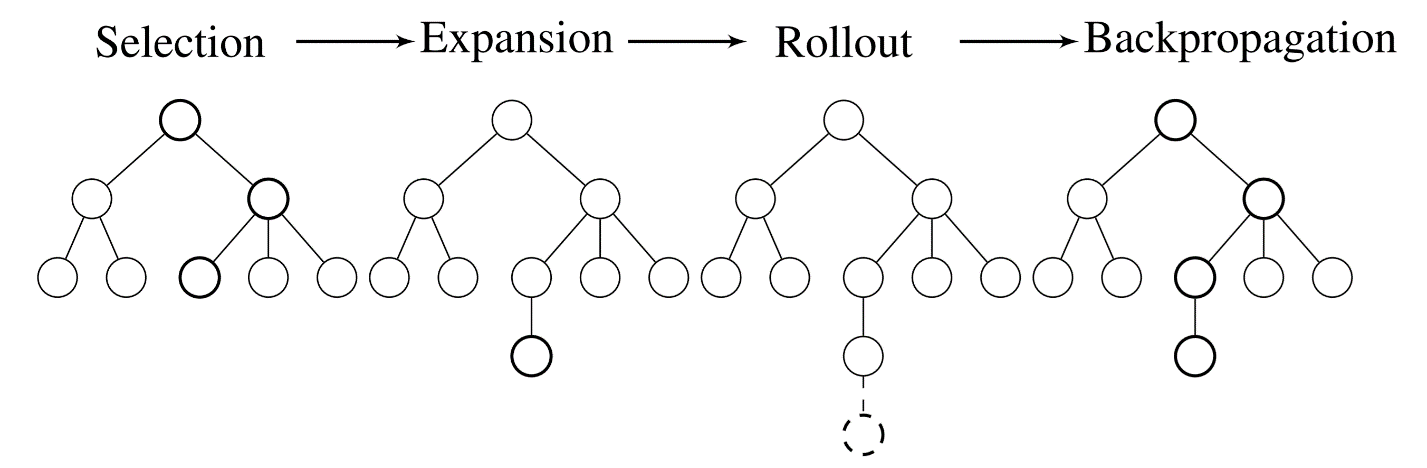
\includegraphics[scale=.825]{figures/MCTS}
\end{figure}
Instead we look for algorithms that approximate the quality of an action in any given state encountered. Monte-Carlo Tree Search (MCTS) is the premier quality estimator, which estimates via sampling full sequences of the game through self-play and averaging them together (Gelly et al., 2012). By performing rollouts (full simulations of the game from the current state), we build a tree which will eventually contain the optimal value estimates. Thus, MCTS has a very useful property, consistency. Given enough time, this sampling algorithm will find the optimal values for all nodes of the tree, and can therefore select the optimal action at the root state (Gelly et al., 2012). After constructing this consistent tree, we simply need to select the action with the highest quality estimate to act optimally. However, because the algorithm is anytime, stopping the algorithm before convergence can lead to suboptimal estimates and thus imperfect policies (Gelly et al., 2012). Therefore, choosing the action of maximum quality may lead us to play sub optimally, because that action has been estimated to have better quality than it does, or other actions with underestimated values are actually better. The study of how to decide between n actions is explored using multi-armed bandit problems (Gelly et al., 2012). 

\subsection{Parallel MCTS}
MCTS is easily parallelisable. We exploit this since we wish to balance the need of sampling the game space to yield decent strategies with the need to decide on the next move within a time interval that human opponents would tolerate. There are three alternatives: leaf parallelisation, root paralellisation and tree parallelisation (Chaslot et al., 2008a). Leaf parallelisation performs multiple parallel roll-outs starting from a leaf node and backpropagates all the results through the tree once all have finished. It is the simplest to implement, but it has a few disadvantages. First of all, the algorithm needs to wait for all threads to finish before backpropagating the results. So it is inefficient in its use of resources. Secondly, it is hard to decide on the exploration term in UCT if the statistics are incremented in steps greater than 1. Root parallelisation involves replicating the whole tree a number of times equal to the number of threads used. The results are combined at the end of the search, before deciding on the next move to make in the real game. It generally performs better than leaf parallelisation, but it requires a good combination of the final results. It is memory inefficient as it stores multiple trees and it duplicates a lot of the effort. Tree parallelisation addresses the above issues by keeping a single copy of the tree and using mutexes to lock the branches accessed by the threads. The locks are global locks, where the whole tree is locked, or local locks, where each node requires the accessing thread to get a lock. The latter has a better overall performance, but only a negligible time decrease. Nonetheless, we have chosen a tree parallelisation with local mutexes due to its advantages over leaf or root parallelisations. A lock-free version implementation (Silver et al., 2016; Chaslot et al., 2008a) is straightforward to write, but it would probably provide a minor improvement in speed while sacrificing a number of results. Our agents run a relatively small number of iterations compared to other applications of MCTS (e.g. AlphaGo Silver et al., 2016), so we wanted a synchronised approach to avoid any overwrites. To reduce the overhead caused by the synchronisation, we are also using virtual loss to discourage multiple threads from following the same path through the tree.

\subsection{Multi-armed Bandits}
A multi-armed bandit problem \cite{robbins1952} is a sequential decision problem over a set of possible actions ("arms"). At each time step, the player pulls one of the arms and recieves a pre-allocated and observable reward. The goal is to maximize the rewards obtained over a sequence of allocations and actions. The term multi-armed bandit comes from the sequential decision problem of playing multiple slot machines at once (the slot machines being the “multi-armed bandit”), and repeatedly choosing which arm to pull next. The player must balance the exploitation of arms that did well in the past and the exploration of arms that are currently underestimated but which may give higher payoffs in the future. 
When playing board games using reinforcement learning, each decision is made by simulating and evaluating as many possible game rollouts from the current state as time and resources allow. Algorithms for bandits (more specifically, for a tree-based version of the bandit problem) can be used to explore more efficiently the huge tree built by simulating game rollouts by focusing on the most promising subtrees (i.e. where the sampled return was greatest). A crucial algorithm in the literature, the UCT algorithm for hierarchical bandits of Kocsis and Szepesvari [2006] \cite{Kocsis2006}, which can be seen as an extenion of the UCB bandit algorithm, is directly applicable to these tree-based searches. UCT has demonstrable improvements over prior methods such as \(\epsilon\)-greedy, where the optimal action is selected with probability 1-\(\epsilon\) and a uniformly random action with the remaining probability \(\epsilon\). UCT is proven to converge to optimal and consistent decisions as the number of samples grows to infinity (Kocsis and Szepesvri 2006). The main idea is to bias the MCTS to bias search towards actions which have been tried he least number of times and therefore are the most uncertain (Gelly et al., 2012). This is an extension to the natural idea that one must balance between exploration (trying new actions) and exploitation (selecting the action of highest quality). These improvements stem from analyzing the regret of a player who pulls the arms according to some strategy. We can make comparisons between this strategy's performance with that of an optimal strategy that, for any n step horizon, consistently plays the best arm. Stated more simply, we analyze the regret of a player who does not always play optimally. This regret is typically formulated as follows:

\begin{equation}
R_n \defeq \max_{i=1,...,K} \sum_{t=1}^n X_{i,t} - \sum_{t=1}^n X_{I_t,t}
\end{equation}

Where we have K \(\geq\) 2 arms and sequences of rewards \(X_{i,1},X_{i,2}...\) associated with each arm \( i = 1,...,K\). Where at each time step \( t=1,...,N\) the player selects an arm \(I_t\) and recieves the pre-allocated reward \(X_{I_t,t}\).

The successes of UCB, and in turn the UCT algorithm, come from bounding this regret defined above. The UCT algorithm effectively moderates the tradeoff between exploitation and exploration by introducing a bias term which quantifies our uncertainty on the current estimates of the action values.
Though multi-armed bandits have been studied in a plethora of environments we are mainly interested in the stochastic and Markovian settings. These settings apply most directly to tree search and thus planning over actions in complex games. This tree search is a sequential decision problem over states in a finite MDP. Like with multi-armed bandits, the assumptions are that the reward and transition distributions are unknown, and we want to act in the MDP so as to maximize the rewards. Another model, with many applications, is that of sleeping bandits. There, it is assumed that the available actions vary over time. \cite{regretAnalysis} 
Another interesting result is that of Kearns et al. who showed that regardless of the size of the state-space, fixed size trees suffice to find an action at the initial state whose value is within some error \(\epsilon\) of the best action. \cite{Kearns2002}

\subsection{Markov Decision Processes}
Reinforcement learning agents plan to maximize future cumulative return. If we try to define what this means mathematically we get the following sequence of rewards starting from any time step t:
\begin{equation}
R_t = r_{t+1} + r_{t+2} + r_{t+3} + r_{t+4}\ldots = \sum_{k=0}^\infty r_{t+k+1}
\end{equation}
If this sequence were to be infinite or we simply wish to tune how much we care about reward now rather than later it is commonplace to add a discount factor \(\gamma\):
\begin{equation}
R_t = r_{t+1} + \gamma r_{t+2} + \gamma^2 r_{t+3} + \gamma^3 r_{t+4}\ldots = \sum_{k=0}^\infty \gamma^k r_{t+k+1}
\end{equation}
Where \(0 \leq \gamma \leq 1\), with \(\gamma\) = 0 being a myopic agent to \(\gamma\) = 1 being a prudent one. Through interaction with the environment and the observation of these reward signals, the agent tries to maximize a function over the expected rewards. The end goal being to learn a policy that makes optimal decisions. A policy \(\pi\) being a mapping from every state \(s\) to a probability distribution over the action space \(P(A)\) for all \(a\in A\), with the probabilities being indirect measures of the value of each action \(a\) in state \(s\). 
To formalize the agent, its interactions with the environment, and the rewards it receives we can model it as a Markov Decision Process (MDP). A MDP is a sequential learning task that satisfies the Markov property: the next state and expected reward are dependent only on the current state and the action chosen and not on anything that preceded them (Russell and Norvig, 2009). In other words, the future is independent of the past given the present. Mathematically it means we assume the following factorization:
\begin{equation}
P(s_1, r_1, a_1 \ldots , s_t, r_t, a_t, s_{t+1}, r_{t+1}) = P(s_t, r_t | s_1, r_1, a_1 \ldots , s_{t-1}, r_{t-1}, a_{t-1}) P(s_{t+1}, r_{t+1} | s_t, r_t, a_t)
\end{equation}
Assuming that our process is markovian, we can go on to define the transition and reward probabilities. We define an MDP as a tuple \(<S,A,\mathcal{P},\mathcal{R}>\) of states \(S\), actions \(A\), the transition probabilities \(\mathcal{P}\), and the reward probabilities \(\mathcal{R}\). Where:
\begin{equation}
\mathcal{P}_{s{s^\prime}}^a = Pr(s_{t+1} = {s^\prime} | s_t = s, a_t = a)
\end{equation}
\begin{equation}
\mathcal{R}_{s{s^\prime}}^a = \mathbb{E}[r_{t+1} | s_t = s, s_{t+1} = {s^\prime}, a_t = a]
\end{equation}
Given the above definitions, the Bellman optimality equation (using action value notation) for an MDP is:
\begin{equation}
Q^*(s,a) = \sum_{s^\prime} \mathcal{P}_{s{s^\prime}}^a (\mathcal{R}_{s{s^\prime}}^a + \gamma \max_{a^\prime} Q^*({s^\prime}, {a^\prime}))
\end{equation}
The key here is that we can express values of states in terms of the values of other states. This allows us to 'bootstrap' estimates of our current state's value given estimates of the values of other states in the future. 

\subsection{Partially-observable Markov Decision Processes}
\subsubsection{Definition}


\subsubsection{Methods for POMDPs}
Using exact methods in complex environments is unfeasible as a result of Bellman’s curse of dimensionality. Instead most approaches use sampling methods (Kurniawati et al., 2008; Silver and Veness, 2010; Somani et al., 2013) or plan using an abstract representation of the belief (Kaelbling and Lozano-Prez, 2013). 

We can divide the most popular POMDP algorithms into three classes: sampling of determinizations, information sets, and belief states. Simply put, determinizations are the process of sampling fully observable states that are possible given the history of the game (belief) and performing Monte Carlo Tree Search on these samples of perfect information. However, this has two major weaknesses pointed out by (Cowling et. al, 2012): strategy fusion and duplication of work. 
\\
\\
\textbf{Strategy fusion:} The algorithm makes the flawed assumption that the same decisions can be made across determinizations, though this is demonstrably false, and as such leads to the fusion of different strategies from each determinization.
\\
\\
\textbf{Duplication of work:} Many of the determinizations will share common nodes, yet this is not exploited, and so work is duplicated across samples.
\\

In an attempt to sidestep these problems, (Cowling et. al, 2012) developed an MCTS algorithm that operated on information sets of states instead of sampled determinizations. This information set approach avoids the duplication problem by keeping track of all possible true states in one tree, however, strategy fusion is still an issue because the rollouts are still sampled via determinizations of the information set. To address this weakness, they proposed a new UCT rule that takes into account the number of times the action was legal in any given determinization. Further, they proposed an extension to ISMCTS to account for the beliefs of the other agents with multiple observer ISMCTS (MO-ISMCTS). However, this increases computational complexity because of the need to store and reason over multiple information set trees. While this is not of particular salience to Settlers of Catan (Dobre, 2018), in the game of Cluedo it is highly strategic to act in correspondence with the belief states of other agents. This can be demonstrated by considering which cards you wish to suggest, taking into account that bluffing is a profitable strategy under certain circumstances, or which cards have been shown to a suggester by a third agent. As mentioned previously, this dissertation is highly influenced by the work of (Silver and Veness, 2010) on planning in large POMDPs, and the thesis of (Dobre, 2018) which explores low-resource learning in complex games. Both of these papers explore planning in the belief state space, which is conceptually very similar to that of information sets. Belief states can be represented by particle filters (Silver and Veness, 2010), factored representations (Dobre, 2018) and though not explored here, hidden markov models/ Dynamic Bayesian networks (Russel and Norvig 2009). POMCP and ISMCTS both sample a fully observable state from the current belief state, then mask out the illegal (impossible) parts of the tree (Dobre, 2018). The number of samples required by these algorithms scales with the support of the belief distribution and its entropy. Because they work with determinizations, both algorithms effectively consist of two sampling phases, one to estimate the current belief and one to estimate the expected return for each sample. This is disadvantageous and incurs increased computational complexity. In contrast, BMCTS does not sample fully observable, but rather propagates the belief in the tree stage and approaches the problem of strategy fusion in the same way as ISMCTS; by modifying the UCT calculations to account for action legality. Dobre’s algorithm plans in an almost exact representation of the belief by making use of a factored representation (Paquet et al., 2005; Williams, 2005). The propagation of belief however requires additional computational load. In an effort to see if this extra complexity was warranted, Dobre experimented with sampling fully observable states at leaf nodes and performing rollouts just like POMCP and ISMCTS; this agent is called, BMCTS with Observable Rollouts (BMCTSOR). It turned out that this agent which worked with observable rollouts outperformed the agent which planned entirely in the belief space. We follow Dobre in using the standard POMDP framework to present the algorithms and make the assumption that the opponents have the same strategy as our own agent, i.e. trying to maximise their expected return. This is known as self-play.
Another huge contribution of the prior literature is the use of action types instead of finer grained actions in the Monte Carlo tree. This hierarchical approach is necessary for two reasons: it simplifies the branching factor, and accounts for any differences between the cardinality of different action types. For example, the end turn action type has only cardinality of one, yet the action type move has a cardinality equal to the number of combinations of legal moves within the dice roll limit. This leads to an imbalance in our agent sampling more move actions over the action of ending the turn. While this may not be such an issue in the game of Cluedo where the action space is rather limited, it certainly is for games where many consecutive actions are possible. In fact, it is never optimal to end your turn in Cluedo if there is still a possible action to be taken. So we abstracted the action space further by removing ‘end turn’ as an action and we instead automatically end the turn when the player has no more possible actions to take.

\section{Cluedo}
Cluedo is a complex, non-cooperative game of imperfect information where turns are taken sequentially and the goal of the game is symmetric; to reduce the entropy about the contents of the envelope enough to accurately accuse the correct weapon/suspect/room tuple. The game is also non-deterministic, following from the dice rolls. The imperfect information comes into play when a player observes (but is not a participant in) a suggestion and a succeeding falsification of said suggestion. Inductively reasoning about these observations are of high strategic importance for an optimal Cluedo agent yet are also not a necessity for winning. Unless you assume all the other agents are optimal inductive reasoners, in which case a lucky accusation is the only avenue to win in the absence of information gathering from the aforementioned observations. This is because the goal of the game can be abstracted from correctly accusing, to a race to reduce entropy. This follows from the fact that reducing entropy to zero effectively means that you know the location of every card. Subsequently, any information which can lead to a reduction in entropy about the contents of the envelope must be taken advantage of. This includes the content of suggestions, which can inform a player about the suggester’s hand/intentions, if you reason about player types. Computation becomes increasingly expensive as the model reasons over nested beliefs and different player types. Due to time restrictions, we leave the avenue of reasoning over player types (and thus induction about the contents of a suggestion) to future work. 

Even more information however can be gleaned from the observation of who falsified the suggestion in conjunction with the content of the suggestion. If a suggestion has been falsified by another agent, it can be said with absolute certainty that said agent has one of the three cards suggested. If through keeping track of our belief of where all cards are, we already know that two of the cards are accounted for (and not in the hand of the falsifier), we can deduce that the falsifier’s hand contains the final card. On the other hand, if only one or none of the cards are accounted for then we can still update our beliefs via a Bayesian update given the probabilities of an observation and the probability of the observation given the pmf of each suggested card. This improvement indeed saw increased performance for our heuristic agent compared to the same agent who does not reason over partially observable interactions. Choosing which cards to suggest too has strategic importance, as mentioned before other players can reason about your hand based off of your suggestions. Since we deferred to address this type of reasoning, we here also defer strategically suggesting in order to avoid revealing information or misleading other players about the agent’s hand. Instead, our most advanced agent simply suggests the tuple with highest entropy. 

Taking a turn in Cluedo is where the complexity of the game creeps in due to turns consisting of one or two actions respectively. At the same time however, the game rules lend themselves to a natural hierarchy of action-types over the action space and the action types are further subdivided into two distinct yet flexible main phases of a turn. At the beginning of each player’s turn the optimal play is to accuse if you have sufficient knowledge of the envelope or to move instead. A slight simplification we made to reduce action space complexity was to only allow accusations in this beginning phase as the alternative, to also allow an accusation after a move, is redundant because a move itself provides no information and thus the two sequences are equivalent in terms of belief. Per the rules an agent cannot suggest in this first stage of a turn unless in the intermediate play between turns, the character their token represents has been suggested and thus moved to the suggested room. The second phase of a turn is then conditional on two factors: the first phase action was a move, and that move left the player’s token in a room. If both conditions are met, a player may then suggest their current room and any weapon-suspect pair they choose. This regular structure in turn taking leads into predictable sequences of moves and suggestions until an agent is confident enough to accuse. None of our implemented heuristic agents accuse until the entropy of the envelope is zero. While a human may accuse earlier due to an overly optimistic strategy or based on some knowledge of their opponents’ player types and suggestion histories. 

\section{CluedoSim}
\begin{figure}[h]
\caption{The CluedoSim environment (left: only heuristic agents, right: 3 heuristic agents and a human player)}
\centering
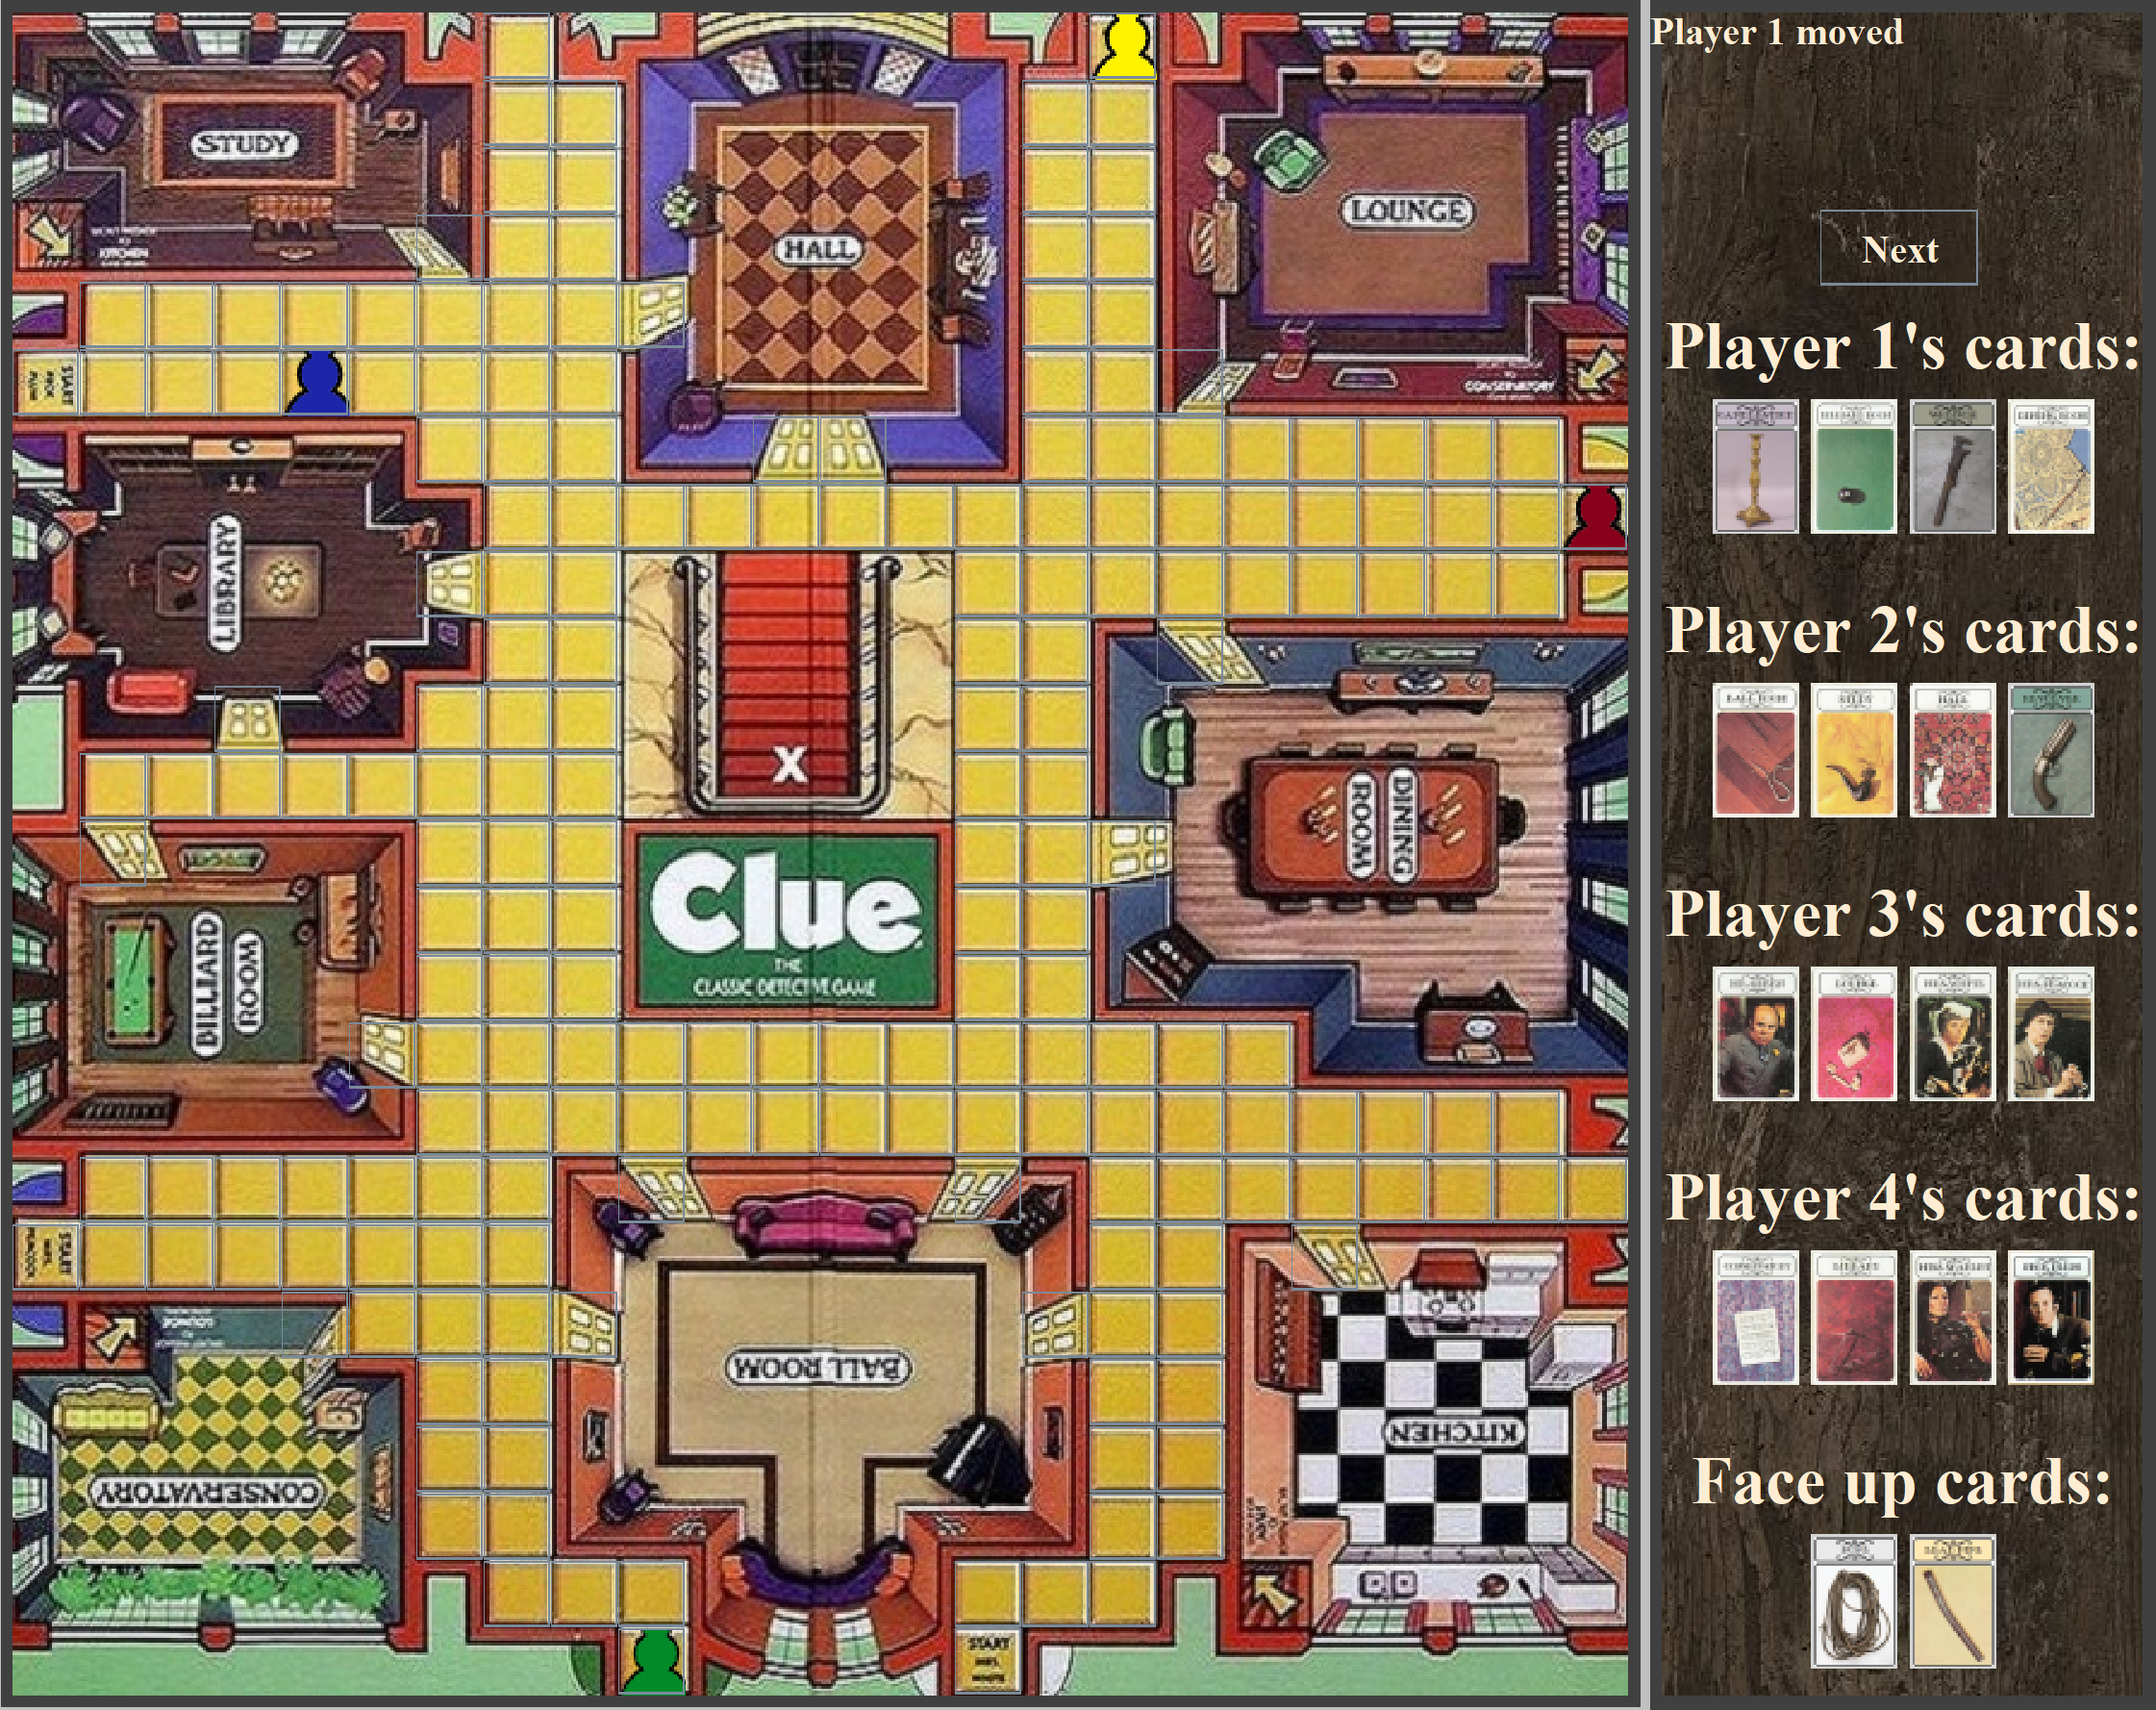
\includegraphics[scale=.3]{figures/cluedoSim}
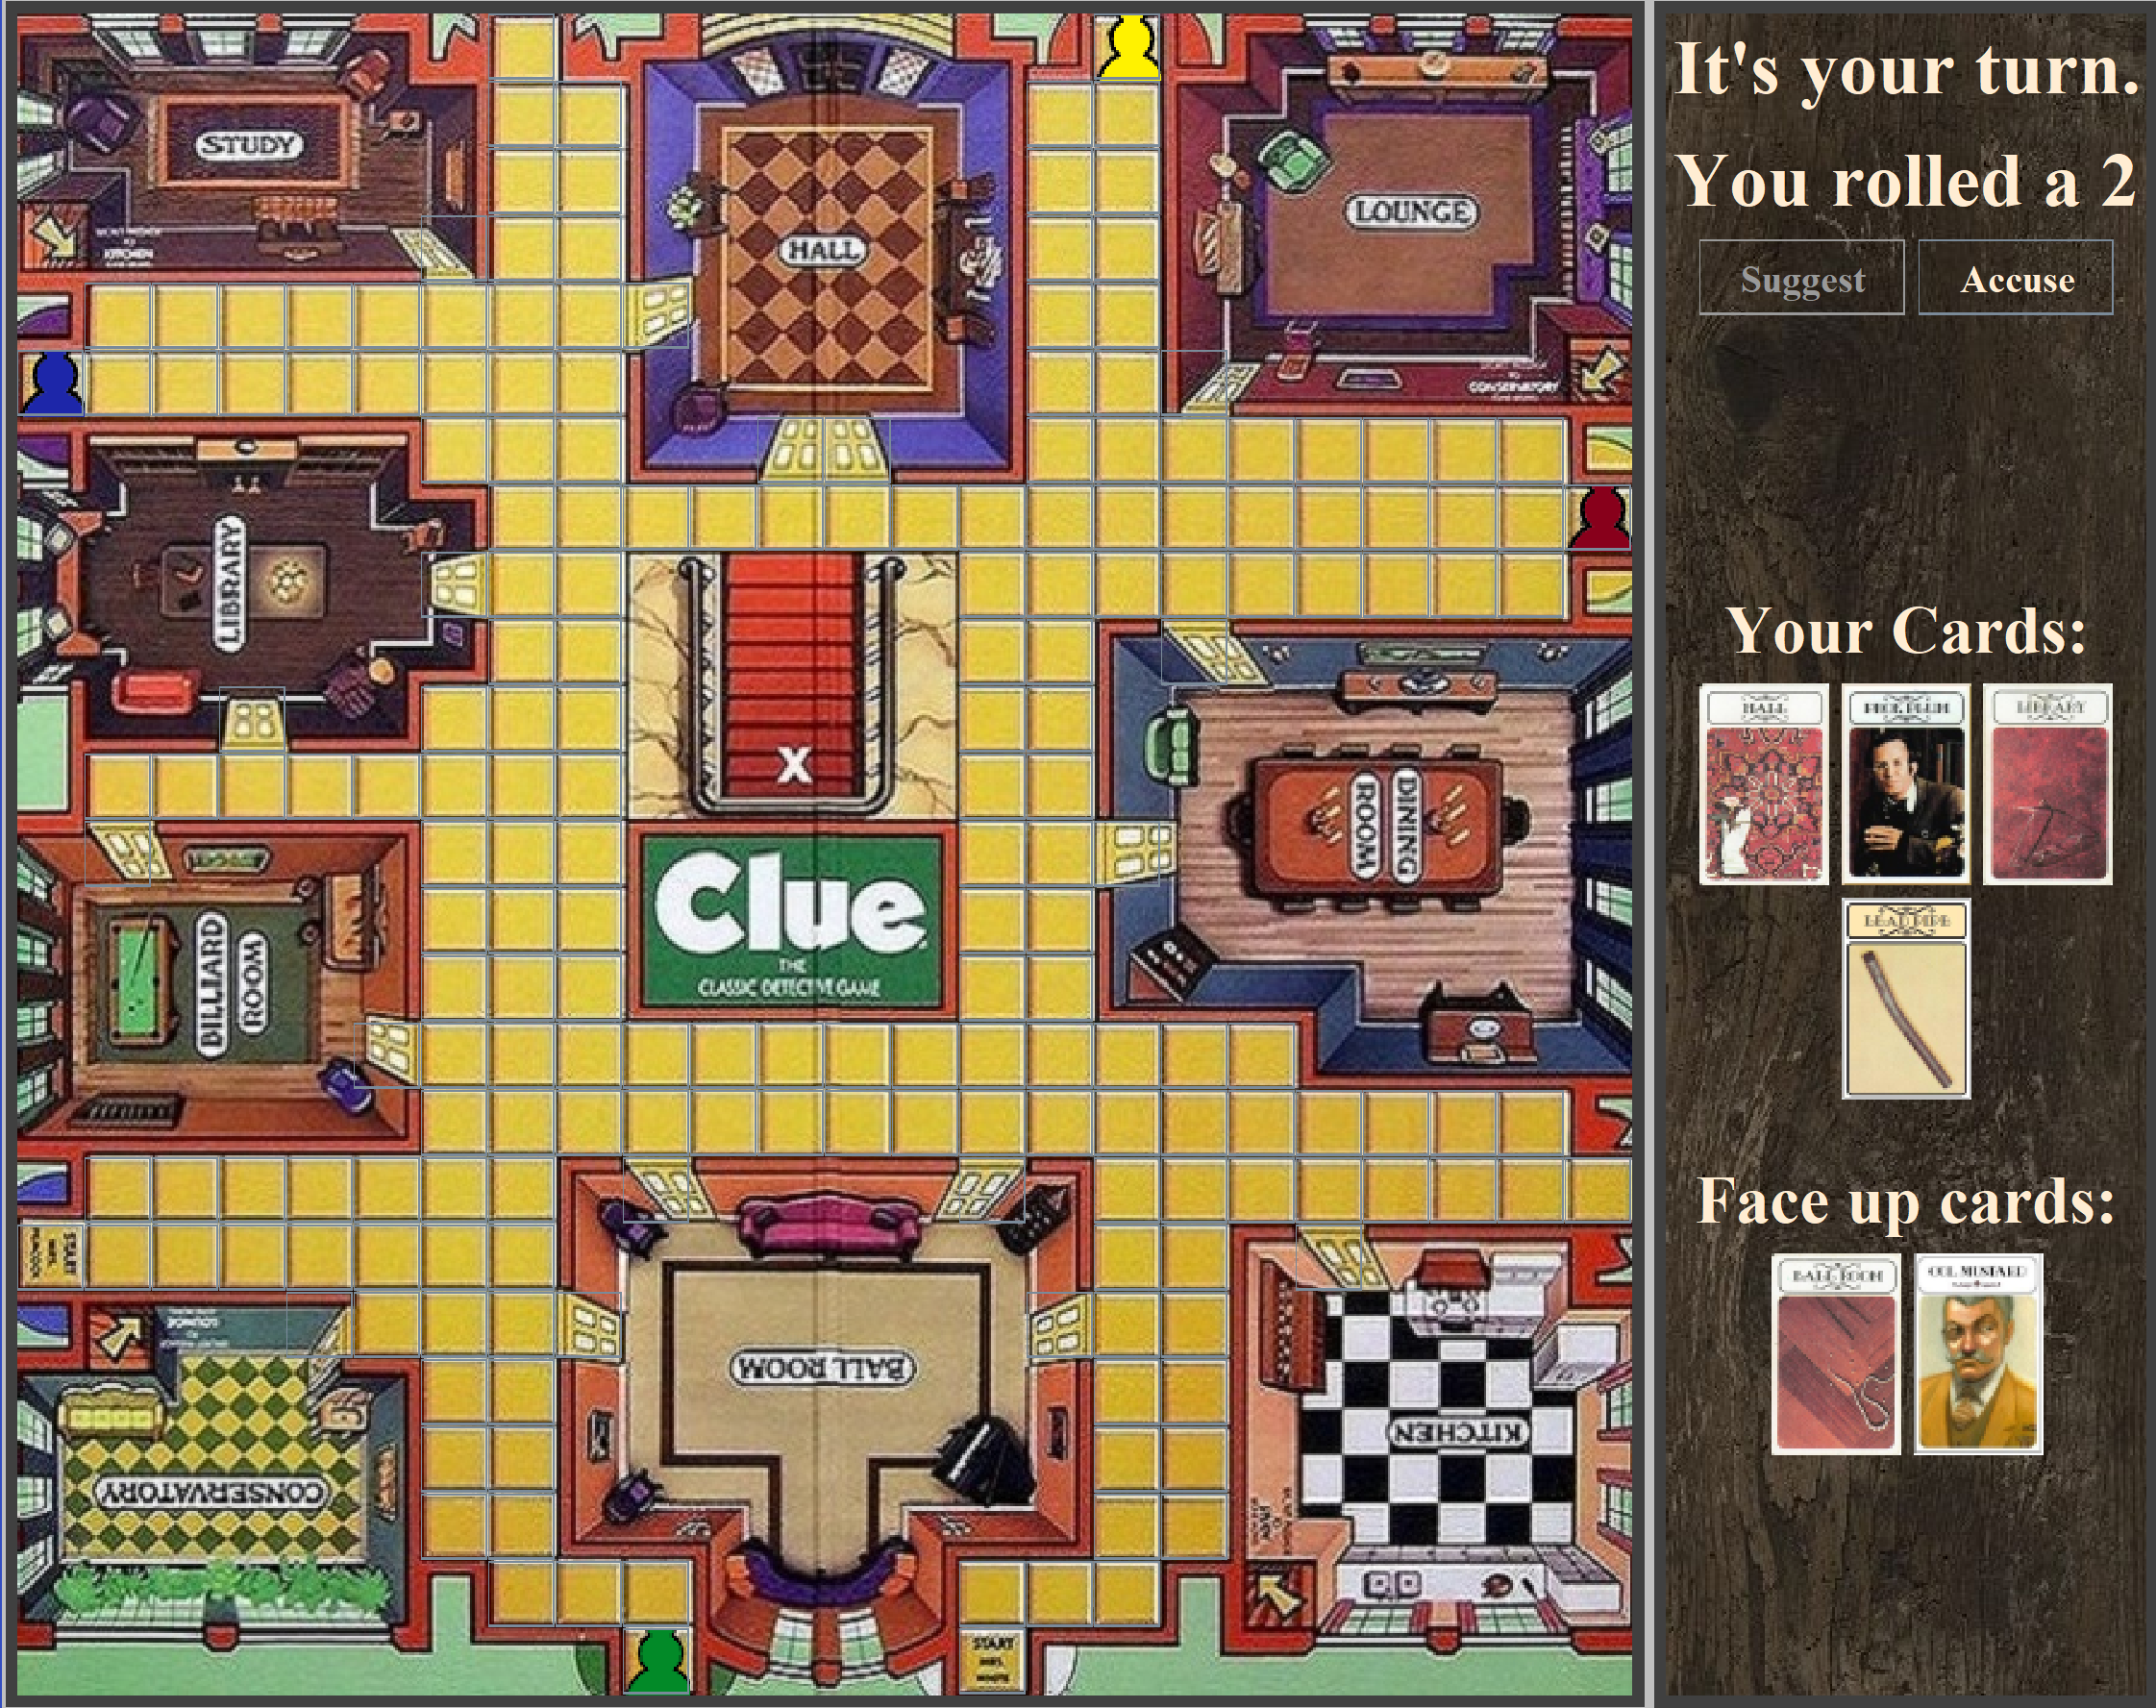
\includegraphics[scale=.3]{figures/humanCluedoSim}
\end{figure}

The first step was to build a simulator for the game with which we could test our agents against each other and time permitting, measure them against human performance. With this end in mind, and also for testing purposes, a GUI was necessary and was assembled using Java’s Swing package. The game logic and heuristic agents were also coded in Java and communicate via a player interface which allows for easy extension or implementation of new agents. It was also necessary to use a database to log game-specific info and also record the results of many games. This was achieved using MongoDB. 

\subsection{Heuristic agent}
The heuristic agent combines the AStar algorithm for path finding and an entropy centered heuristic for suggestions. The agent always aims to suggest the room/weapon/suspect tuple with highest current entropy. Explicit probabilities for each card are kept and updated after observations from other agents (when any suggestion is proved false). When the observation is partially observable, i.e. when the agent is neither the suggester nor falsifier, the agent updates the card probabilities using Bayes rule.




\newpage
\bibliography{references} 
\nocite{*}
\bibliographystyle{IEEEtran}

\end{document}

